\documentclass[12pt,a4paper]{article}

\usepackage[T1]{fontenc}
\usepackage[utf8]{inputenc}
\usepackage[english]{babel}
\usepackage{booktabs}
\usepackage{graphicx}
\usepackage{hyperref}
\usepackage{caption}
\usepackage{float}
\usepackage{geometry}
\usepackage{listings}
\usepackage{xcolor}
\usepackage{amsmath}
\usepackage{array}
\usepackage{multirow}
\usepackage{pgfplots}
\pgfplotsset{compat=1.18}

\geometry{
  a4paper,
  top=2.5cm,
  bottom=2.5cm,
  left=2.5cm,
  right=2.5cm
}

\hypersetup{
  colorlinks=true,
  linkcolor=blue,
  urlcolor=blue,
  citecolor=blue
}

\lstset{
  basicstyle=\ttfamily\small,
  breaklines=true,
  frame=single,
  backgroundcolor=\color{gray!10}
}

\title{
  \textbf{Scale-Up Analytics: DuckDB vs Apache Spark} \\
  \large Comparing Scale-Up and Scale-Out Approaches \\
  on the TPC-H 100~GB Benchmark
}
\author{Franciszek Job \and Przemys\l{}aw Popowski}
\date{\today}

\begin{document}

\maketitle

\begin{abstract}
This report presents an empirical comparison of two approaches to large-scale data
analytics: \textbf{scale-up} using DuckDB on a single HPC node of the Ares cluster
(PLGrid) and \textbf{scale-out} using Apache Spark on an AWS EMR cluster. Both
environments are allocated an equivalent amount of RAM ($\approx$128~GB). The benchmark
is based on the TPC-H dataset at scale factor~100 (approximately 100~GB of input data
in Parquet format). Six representative SQL queries (Q1, Q3, Q5, Q6, Q10, Q21) were
executed, each in 4 runs (the first \textit{cold} run was discarded; the remaining
3 warm runs were used in the analysis). DuckDB achieved execution times in the range
of 12--31~seconds, while Spark ranged from 3 to 56~seconds. Each engine won in exactly
3 out of 6 queries: Spark dominated in scans and simple aggregations (Q1, Q6, Q10),
while DuckDB outperformed in complex joins and correlated subqueries (Q3, Q5, Q21).
\end{abstract}

\tableofcontents
\newpage

% ============================================================
\section{Introduction}
% ============================================================

As the volume of data generated by organizations continues to grow, choosing the right
analytical processing architecture becomes a critical engineering decision. The
traditional \textit{scale-out} approach, represented by systems such as Apache
Hadoop/Spark, distributes the workload across multiple compute nodes. An alternative
is the \textit{scale-up} approach --- using a single, powerful server with a large
amount of RAM and a modern analytical engine.

\subsection{Motivation}

The increasing availability of ``fat node'' servers (256--1024~GB RAM) and the
emergence of high-performance in-memory engines such as DuckDB~\cite{duckdb2019} have
made the scale-up approach increasingly attractive. DuckDB implements vectorized
columnar query execution and is capable of efficiently processing hundreds of
gigabytes of data without the need to manage a cluster.

\subsection{Research Question}

This report addresses the question: \textit{can a single HPC node running DuckDB
compete with an Apache Spark cluster, given equivalent memory resources?} The
hypothesis is that for data fitting in RAM, DuckDB will be comparable to or faster
than Spark, due to the absence of network communication overhead and cluster
management costs.

\subsection{Scope}

\begin{itemize}
  \item Generation and processing of TPC-H data at scale factor 100 ($\approx$100~GB)
  \item Environment setup: DuckDB on a PLGrid HPC node and Spark on AWS EMR
  \item Execution of 6 benchmark queries (Q1, Q3, Q5, Q6, Q10, Q21)
  \item Analysis of results, costs, and development of a decision framework
\end{itemize}

% ============================================================
\section{Test Environment}
% ============================================================

\subsection{HPC Node --- Scale-Up (DuckDB)}

The scale-up experiments were conducted on a compute node of the Ares cluster at
Cyfronet AGH, accessible through the PLGrid infrastructure.

\begin{table}[H]
  \caption{HPC Node Specification (Scale-Up)}
  \label{tab:hpc-spec}
  \begin{tabular}{ll}
    \toprule
    \textbf{Parameter} & \textbf{Value} \\
    \midrule
    System              & Ares, Cyfronet AGH (PLGrid) \\
    SLURM partition     & \texttt{plgrid} \\
    vCPU count          & 8 \\
    Total RAM           & 187~GB \\
    RAM for DuckDB      & 128~GB \\
    Filesystem          & NFS Lustre (\texttt{/net/pr2}) \\
    Operating system    & Linux \\
    Python              & 3.11 \\
    DuckDB              & 0.10+ \\
    Data format         & Parquet \\
    \bottomrule
  \end{tabular}
\end{table}

\subsection{AWS EMR Cluster --- Scale-Out (Spark)}

The scale-out environment was built on an Amazon EMR cluster, with hardware
configuration matched to the HPC node (equivalent RAM).

The entire setup was run within AWS Academy Learner Lab (university account):
access restricted to the \texttt{us-east-1} region, temporary STS credentials
refreshed each session ($\approx$4~h), and academic credit pool instead of
card-based billing.

\begin{table}[H]
  \centering
  \caption{AWS EMR Cluster Specification (Scale-Out)}
  \label{tab:emr-spec}
  \begin{tabular}{ll}
    \toprule
    \textbf{Parameter} & \textbf{Value} \\
    \midrule
    EMR version              & 7.1.0 \\
    Region                   & us-east-1 \\
    Master node              & m5.xlarge (16~GB RAM, 4~vCPU) \\
    Core nodes (compute)     & 3$\times$ m5.4xlarge (192~GB RAM, 48~vCPU) \\
    Total RAM (core nodes)   & 192~GB \\
    RAM for Apache Spark     & 128~GB \\
    Storage                  & Amazon S3 \\
    Apache Spark             & 3.5 \\
    \texttt{spark.executor.memory}       & 16g \\
    \texttt{spark.executor.cores}        & 4 \\
    \texttt{spark.executor.instances}    & 8 \\
    \texttt{spark.sql.shuffle.partitions} & 200 \\
    Adaptive Query Execution & enabled \\
    \bottomrule
  \end{tabular}
\end{table}

\subsection{Hardware Equivalence Principle}

The key assumption of this benchmark is matching memory resources: both environments
have $\approx$128~GB RAM available for the analytical engine. The EMR master node
does not participate in computations and is excluded from the comparison.

% ============================================================
\section{Test Data --- TPC-H 100~GB}
% ============================================================

\subsection{TPC-H Standard}

TPC-H~\cite{tpch} is a widely used benchmark for Decision Support Systems. The dataset
models an order database of a wholesale supplier with 8 tables of varying sizes. The
scale factor (SF) parameter determines the data scale: SF~=~1 corresponds to
$\approx$1~GB, and SF~=~100 corresponds to $\approx$100~GB of raw data.

\subsection{Data Generation}

On the scale-out side (Spark/EMR), data was generated using \texttt{tpch-dbgen}
(repository \texttt{electrum/tpch-dbgen}) compiled directly on the EMR master node.
Large tables were split into parts and streamed to S3 (\texttt{lineitem} in 3 parts,
\texttt{-C~3}; \texttt{partsupp} in 2 parts, \texttt{-C~2}) to fit within the
master's local disk space. Raw \texttt{.tbl} files (pipe-separated values) were
uploaded to an S3 bucket, where Apache Spark converted them to Parquet format with
ZSTD compression. On the scale-up side (DuckDB/HPC), an equivalent dataset was
generated and used independently on the Ares compute node.

\begin{table}[H]
  \centering
  \caption{TPC-H Table Sizes at SF=100}
  \label{tab:tpch-sizes}
  \begin{tabular}{lrrl}
    \toprule
    \textbf{Table} & \textbf{Rows} & \textbf{Size (.tbl)} & \textbf{Description} \\
    \midrule
    \texttt{lineitem}  & $\approx$600M & $\approx$68~GB  & Order line items (primary) \\
    \texttt{orders}    & $\approx$150M & $\approx$15~GB  & Orders \\
    \texttt{partsupp}  & $\approx$80M  & $\approx$10~GB  & Part-supplier combinations \\
    \texttt{customer}  & $\approx$15M  & $\approx$2.3~GB & Customers \\
    \texttt{part}      & $\approx$20M  & $\approx$2.3~GB & Parts \\
    \texttt{supplier}  & $\approx$1M   & $\approx$136~MB & Suppliers \\
    \texttt{nation}    & 25            & $<$1~MB         & Nations \\
    \texttt{region}    & 5             & $<$1~MB         & Regions \\
    \midrule
    \textbf{Total}     &               & $\approx$100~GB & \\
    \bottomrule
  \end{tabular}
\end{table}

% ============================================================
\section{Benchmark Methodology}
% ============================================================

\subsection{Query Selection}

Six queries were selected from the official TPC-H set of 22, representing different
computational patterns:

\begin{table}[H]
  \centering
  \caption{Selected TPC-H Queries}
  \label{tab:queries}
  \begin{tabular}{clll}
    \toprule
    \textbf{No.} & \textbf{Name} & \textbf{Pattern} & \textbf{Rationale} \\
    \midrule
    Q1  & Pricing Summary       & Aggregation on $\approx$68~GB     & Pure aggregation, ideal for DuckDB \\
    Q3  & Shipping Priority     & 3-table JOIN + grouping           & Classic OLAP join \\
    Q5  & Local Supplier Volume & 6-table JOIN                      & Complex multi-join \\
    Q6  & Revenue Change        & Filter + aggregation              & IO-bound, simple arithmetic \\
    Q10 & Returned Item Rep.    & 4-table JOIN + filter             & Grouped analysis \\
    Q21 & Suppliers Waiting     & EXISTS / NOT EXISTS               & Correlated subqueries \\
    \bottomrule
  \end{tabular}
\end{table}

% ============================================================
\section{Results}
% ============================================================

\subsection{Execution Times}

\begin{table}[H]
  \centering
  \caption{TPC-H Query Execution Times --- DuckDB vs Spark [seconds]}
  \label{tab:results}
  \begin{tabular}{lrrrr|rrrr|r}
    \toprule
    & \multicolumn{4}{c|}{\textbf{DuckDB (HPC)}} & \multicolumn{4}{c|}{\textbf{Spark (EMR)}} & \textbf{Speedup} \\
    \textbf{Query} & min & mean & max & std & min & mean & max & std & Duck/Spark \\
    \midrule
    Q1  & 17.90 & 18.49 & 19.38 & 0.78 &  8.89 &  9.35 &  9.89 & 0.50 & 1.98 \\
    Q3  & 15.13 & 15.59 & 15.91 & 0.41 & 15.94 & 16.16 & 16.40 & 0.23 & 0.96 \\
    Q5  & 16.03 & 17.20 & 19.09 & 1.65 & 26.46 & 26.79 & 27.11 & 0.33 & 0.64 \\
    Q6  & 11.56 & 12.04 & 12.57 & 0.51 &  2.91 &  3.07 &  3.34 & 0.23 & 3.92 \\
    Q10 & 25.01 & 25.17 & 25.26 & 0.14 & 13.97 & 14.01 & 14.08 & 0.06 & 1.80 \\
    Q21 & 29.92 & 31.30 & 33.30 & 1.77 & 54.71 & 55.36 & 55.75 & 0.57 & 0.57 \\
    \bottomrule
  \end{tabular}
\end{table}

\subsection{Observations}

The results show clear variation depending on the nature of the query. DuckDB wins
in 3 out of 6 cases (Q3, Q5, Q21), while Spark wins in the remaining 3 (Q1, Q6, Q10).

\begin{itemize}
  \item \textbf{Q6} --- largest Spark advantage (4$\times$ faster, 3.07~s vs 12.04~s).
        Simple range-predicate filtering on \texttt{lineitem} --- Spark efficiently
        scans columnar data from S3, and Adaptive Query Execution (AQE) dynamically
        optimizes execution and reduces the number of partitions.
  \item \textbf{Q1} --- Spark 2$\times$ faster (9.35~s vs 18.49~s).
        Full scan of \texttt{lineitem} with aggregation --- Spark leverages the
        combined parallelism of the cluster (core nodes total 48~vCPU), whereas
        DuckDB is limited to the 8~vCPU of a single node.
  \item \textbf{Q10} --- Spark clearly faster (14.01~s vs 25.17~s, ratio 1.80$\times$).
        4-table JOIN with filtering --- Spark effectively distributes join work
        across nodes in the distributed environment.
  \item \textbf{Q3} --- tie (16.16~s vs 15.59~s, difference $<$4\% in DuckDB's favor).
        Classic OLAP 3-table JOIN --- despite a large disparity in available hardware
        resources, a standalone DuckDB node handles this query as fast as the entire
        Spark cluster.
  \item \textbf{Q5} --- DuckDB over 50\% faster (17.20~s vs 26.79~s).
        6-table JOIN with small dimension tables --- DuckDB efficiently buffers small
        tables in local RAM, avoiding the significant network communication overhead
        incurred by Spark.
  \item \textbf{Q21} --- largest DuckDB advantage (31.30~s vs 55.36~s, Spark overhead
        1.77$\times$). \texttt{EXISTS}/\texttt{NOT EXISTS} subqueries --- DuckDB's
        optimizer converts these into efficient local \textit{semi-join} and
        \textit{anti-join} operations. In Spark, these operations are particularly
        costly due to the requirement for distributed join processing.
\end{itemize}

\subsection{Charts}

\begin{figure}[H]
  \centering
  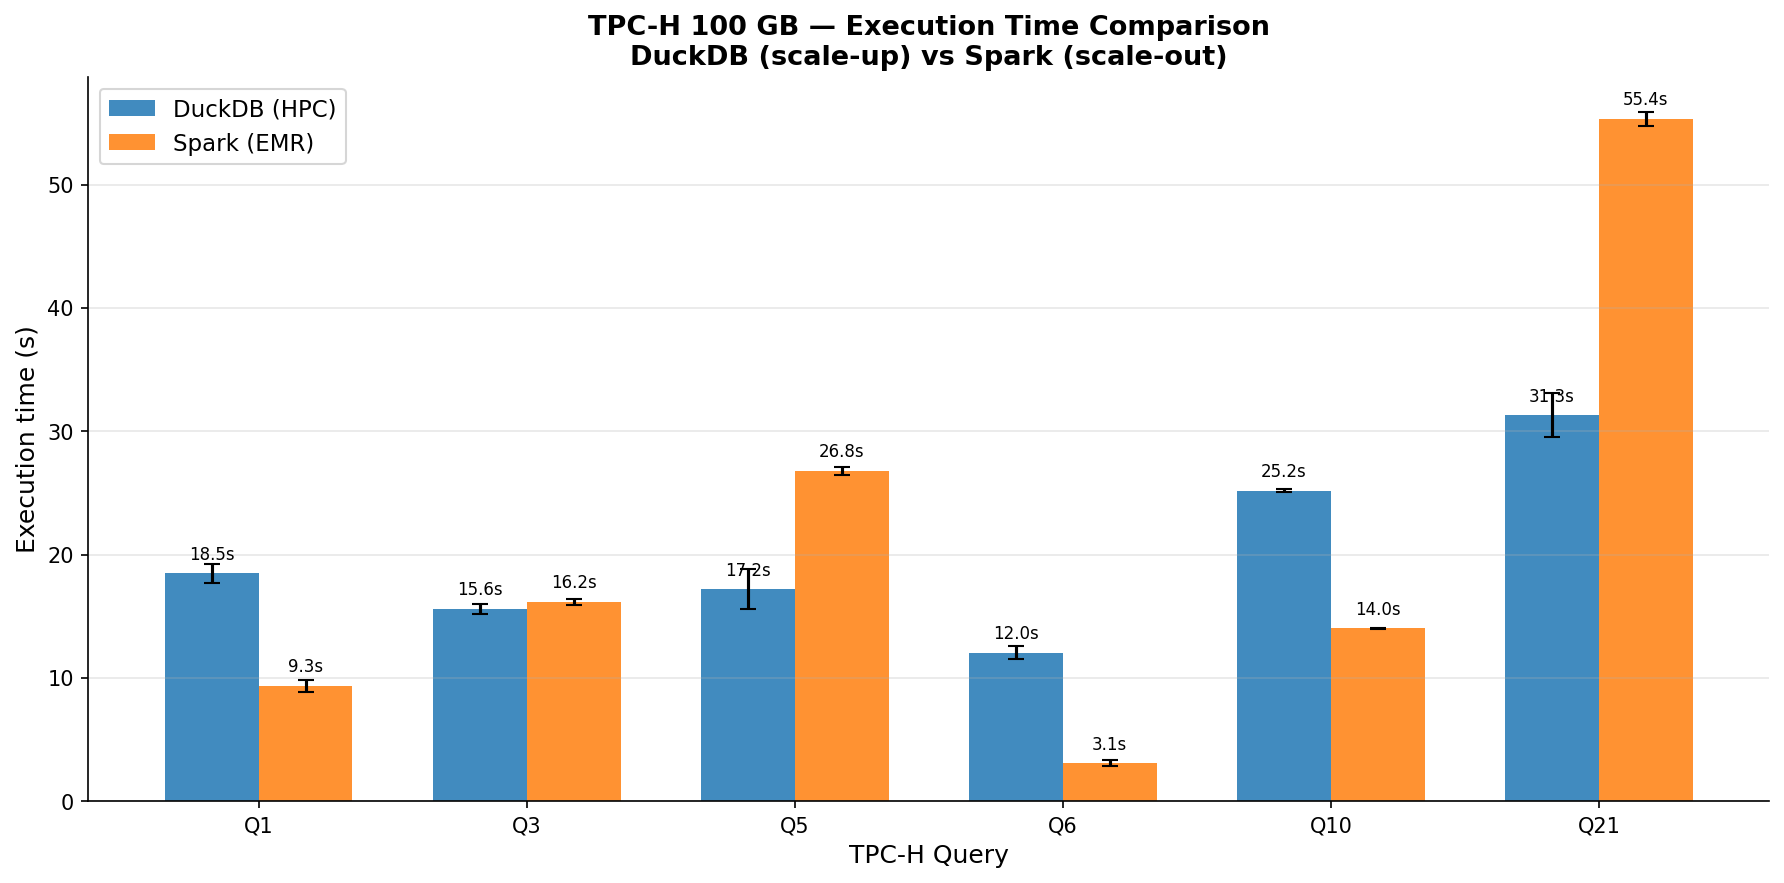
\includegraphics[width=0.9\textwidth]{figures/01_execution_time_comparison.png}
  \caption{Execution time comparison --- DuckDB vs Spark}
  \label{fig:exec-time}
\end{figure}

\begin{figure}[H]
  \centering
  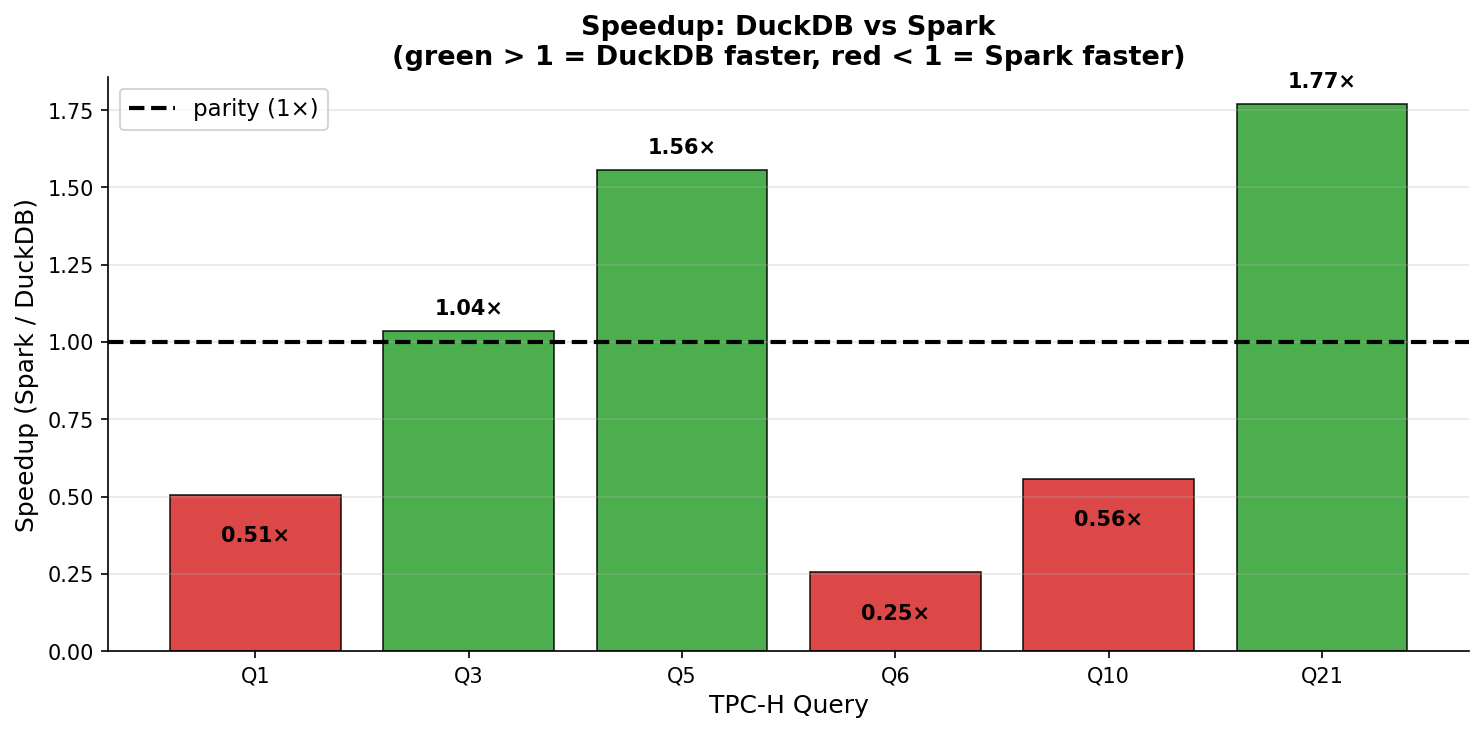
\includegraphics[width=0.8\textwidth]{figures/02_speedup_ratio.png}
  \caption{Speedup ratio DuckDB vs Spark per query (Duck/Spark $>$1 means DuckDB faster)}
  \label{fig:speedup}
\end{figure}

% ============================================================
\section{Analysis}
% ============================================================

\subsection{DuckDB Advantages (Scale-Up)}

DuckDB executes analytical queries using a \textit{push-based vectorized execution}
model with columnar data layout in memory. Key advantages in the context of this
benchmark:

\begin{enumerate}
  \item \textbf{No network overhead} --- data resides in local node memory, no costly
        network shuffle operations
  \item \textbf{SIMD vectorized operations} --- processing batches of rows rather than
        individual tuples
  \item \textbf{Lazy materialization} --- DuckDB avoids copying columns not used in
        later stages of the query plan
  \item \textbf{Low management overhead} --- no resource scheduler, master node,
        ZooKeeper, etc.
\end{enumerate}

\subsection{Spark Advantages (Scale-Out)}

Apache Spark provides value in different scenarios:

\begin{enumerate}
  \item \textbf{Horizontal scalability} --- ability to add nodes when data exceeds the
        RAM of a single server
  \item \textbf{Fault tolerance} --- automatic task re-execution after node failure
  \item \textbf{Distributed joins} --- for very complex plans with multiple large tables,
        Spark can better distribute the workload
  \item \textbf{Ecosystem} --- Spark Streaming, MLlib, GraphX
\end{enumerate}

% ============================================================
\section{Cost Analysis}
% ============================================================

\begin{table}[H]
  \centering
  \caption{Infrastructure Cost Comparison}
  \label{tab:costs}
  \begin{tabular}{llrl}
    \toprule
    \textbf{Option} & \textbf{Estimated cost/h} & \textbf{RAM} & \textbf{Operational overhead} \\
    \midrule
    HPC PLGrid (grant)                          & $\approx$ \$0.00 & 187~GB & low \\
    AWS EMR (m5.xlarge + 3$\times$ m5.4xlarge) & $\approx$ \$2.50 & 192~GB & high \\
    \bottomrule
  \end{tabular}
\end{table}

For datasets that fit entirely in the RAM of a single node (utilization below 80\%
of available memory), the \textit{scale-up} approach (DuckDB) proves not only more
performant but also significantly cheaper and simpler to manage. The EMR cluster
(\textit{scale-out}) introduces additional, often overlooked costs and overheads:

\begin{itemize}
  \item environment startup time ($\approx$20~minutes)
  \item cost of maintaining the \textit{master} node, which performs no direct
        compute tasks
  \item data transfer costs and API call costs to Amazon S3
  \item time spent managing distributed configuration
\end{itemize}

\textbf{Note:} Strict lifecycle management of the cluster is essential. Leaving the
described AWS EMR environment (m5 instance configuration) in idle (\texttt{WAITING})
state over an entire weekend (48~hours) will generate a wasteful cost of approximately
\textbf{\$120}. Automatic cluster termination after benchmark completion is critical
from a budget perspective.

% ============================================================
\section{Conclusions}
% ============================================================

\begin{enumerate}
  \item \textbf{DuckDB is competitive with Apache Spark} given equivalent memory
        resources for datasets of $\approx$100~GB. Query execution times of 12--31~seconds
        are acceptable for interactive analysis.
  \item \textbf{Scale-up has a cost and operational advantage} for data fitting in
        node RAM: no need to manage a cluster, lower setup time, no risk of leaving
        a running (and costly) cluster idle.
  \item \textbf{Scale-out (Spark/EMR) is justified} when data exceeds the RAM of a
        single node, fault tolerance is required, or the workload extends beyond SQL
        analytics (streaming, ML).
  \item \textbf{Recommendation}: start with DuckDB on a single node. Migrate to Spark
        when data exceeds $\approx$1~TB or requirements arise that DuckDB cannot fulfill.
\end{enumerate}

% ============================================================
\begin{thebibliography}{9}

\bibitem{duckdb2019}
Raasveldt, M., \& M\"{u}hleisen, H. (2019).
\textit{DuckDB: an Embeddable Analytical Database}.
SIGMOD '19: International Conference on Management of Data.

\bibitem{tpch}
Transaction Processing Performance Council (2023).
\textit{TPC-H Benchmark Specification, Version 3.0.1}.
\url{http://www.tpc.org/tpch/}

\bibitem{spark2016}
Zaharia, M., et al. (2016).
\textit{Apache Spark: A Unified Engine for Big Data Processing}.
Communications of the ACM, 59(11), 56--65.

\end{thebibliography}

\end{document}
